\documentclass{homework}

\title{Problem Set 8}
\author{Kevin Evans}
\studentid{11571810}
\date{April 20, 2022}
\setclass{Physics}{463}
\usepackage{amssymb}
\usepackage{mathtools}
\usepackage{graphicx}
\usepackage{amsthm}
\usepackage{amsmath}
\usepackage{slashed}
\usepackage{boldline}
\usepackage{physics}
\usepackage{tcolorbox}
\usepackage[inter-unit-product =\cdot]{siunitx}

\usepackage[makeroom]{cancel}
\usepackage{booktabs}
\usepackage{multirow}

\usepackage{times}
\usepackage{mhchem}
\usepackage{mathtools}
\usepackage{tabularx}
\usepackage{listings}


\newcommand{\fm}{\femto\meter}
\newcommand{\solution}{	\vspace{1em} \textit{Solution.} \quad }

\begin{document}
	\maketitle
	\begin{enumerate}
		\item % 7.2
			\textbf{\textit{Free electron energies in reduced zone.}} Consider the free electron energy bands of an fcc crystal lattice in the approximation of an empty lattice, but in the reduced zone scheme in which all $\bvec{k}$'s are transformed to lie in the first Brillouin zone. Plot roughly in the $[111]$ direction the energies of all bands up to six times the lowest band energy at the zone boundary at $\bvec{k}=(2 \pi /a) \left(\frac{1}{2}, \frac{1}{2}, \frac{1}{2}\right)$. Let this be the unit of energy. This problem shows why band edges need not necessarily be at the zone center. Several of the degeneracies (band crossings) will be removed when account is taken of the crystal potential.
			
			% get k along [111]
			\solution
			The unit of energy of $\bvec{k} = (2 \pi/a)(\frac{1}{2}, \frac{1}{2}, \frac{1}{2})$ is \begin{align*}
				\epsilon_k & = \frac{\hbar^2 k^2}{2m} = \frac{4 \pi^2 \hbar^2}{2m a^2} \left(3 \times \frac{1}{4}\right) \\
					& = \frac{12\hbar^2 \pi^2}{8m_e a^2} \\
					& = (9/2) (2 \pi / a)^2 \qquad \text{ (with $\hbar^2/2m=1$)}.
			\end{align*}
			The reciprocal lattice vector for the fcc lattice are \begin{align*}
				\bvec{G} & = v_1 \bvec{b}_1 + v_2 \bvec{b}_2 + v_3 \bvec{b}_3 \tag{2.15} \\
					& = \frac{2 \pi}{a} \left[
						v_1 (-\uvec{x} + \uvec{y} + \uvec{z})
						+ v_2 (\uvec{x} - \uvec{y} + \uvec{z})
						+ v_3 (\uvec{x} + \uvec{y} - \uvec{z})
					\right] \tag{2.36}\\
					& = \frac{2 \pi}{a} \left[
						(-v_1 + v_2 + v_3) \uvec{x}
						+ (v_1 - v_2 + v_3) \uvec{y}
						+ (v_1 + v_2 - v_3) \uvec{z}
					\right].
				\intertext{Using the Bragg condition $(\bvec{k} + \bvec{G})^2 = k^2$ and sorta following p. 176, }
				k^2 & = (\bvec{k} + \bvec{G})^2 \\
					& = \left[
						\frac{2 \pi}{a}
							\left(
								u - v_1 + v_2 + v_3
							\right) \uvec{x}
							+
							\left(
								u + v_1 - v_2 + v_3
							\right) \uvec{y}
							+ 
							\left(
								u + v_1 + v_2 - v_3
							\right) \uvec{z}
					\right]^2.
				\intertext{The energy is then}
				\epsilon(u, v_1, v_2, v_3) & = \frac{\hbar^2 k^2}{2m} \\
					& = \frac{\hbar^2}{2m} \left(\frac{2 \pi}{a}\right)^2 \left[
						\left(u - v_1 + v_2 + v_3\right)^2
						+ \left(u + v_1 - v_2 + v_3\right)^2
						+ \left(u + v_1 + v_2 - v_3\right)^2
					\right], \\
					& \text{ where } u \in \mathbb{R}, v_i \in \mathbb{Z}.
			\end{align*}
		
		\pagebreak
		
			For convenience, I will follow Kittel's advice and choose units such that $\hbar^2/2m=1$. I think now, I can just iterate over the indices $v_i$,
			$$
				\begin{array}{clcc}
					\toprule
					\text{Band} & \text{Plane} & \epsilon(u) & \epsilon(0)\\
					\midrule
					1 & 000 & (2 \pi / a)^2 3 u^2 & 0 \\
					2 & \bar{1}\bar{1}\bar{1} & 3(2 \pi / a)^2 (u-1)^2 & 3(2 \pi / a)^2 \\
					3 & 111 & 3(2 \pi / a)^2 (u+1)^2 & 3(2\pi/a)^2 \\
					4 & 100, 010, 001 & (2 \pi / a)^2 (3u^2 + 2u + 3) & 3(2 \pi / a)^2\\
					5 & \bar{1}00, 0\bar{1}0, 00\bar{1} & (2 \pi / a)^2 (3u^2 - 2u + 3) & 3(2 \pi / a)^2 \\
					6 & 110, 101, 011 & (2 \pi /a)^2 (3u^2 + 4u + 4) & 4(2\pi /a)^2 \\
					7 & \bar{1}\bar{1}0, \bar{1}0\bar{1}, 0\bar{1}\bar{1} & (2 \pi / a)^2(3u^2 -4u + 4) & 4(2 \pi / a)^2 \\
					\bottomrule
				\end{array}
			$$
			After $4(2\pi/a)^2$, we hit the upper limit where the next plane reaches $\epsilon(0)=8(2\pi/a)^2$.
			
			\vspace{2em}
			
			Plotting the seven bands in Desmos (with the $x$-axis scale being from $k=\pm \pi/a$),\begin{center}
				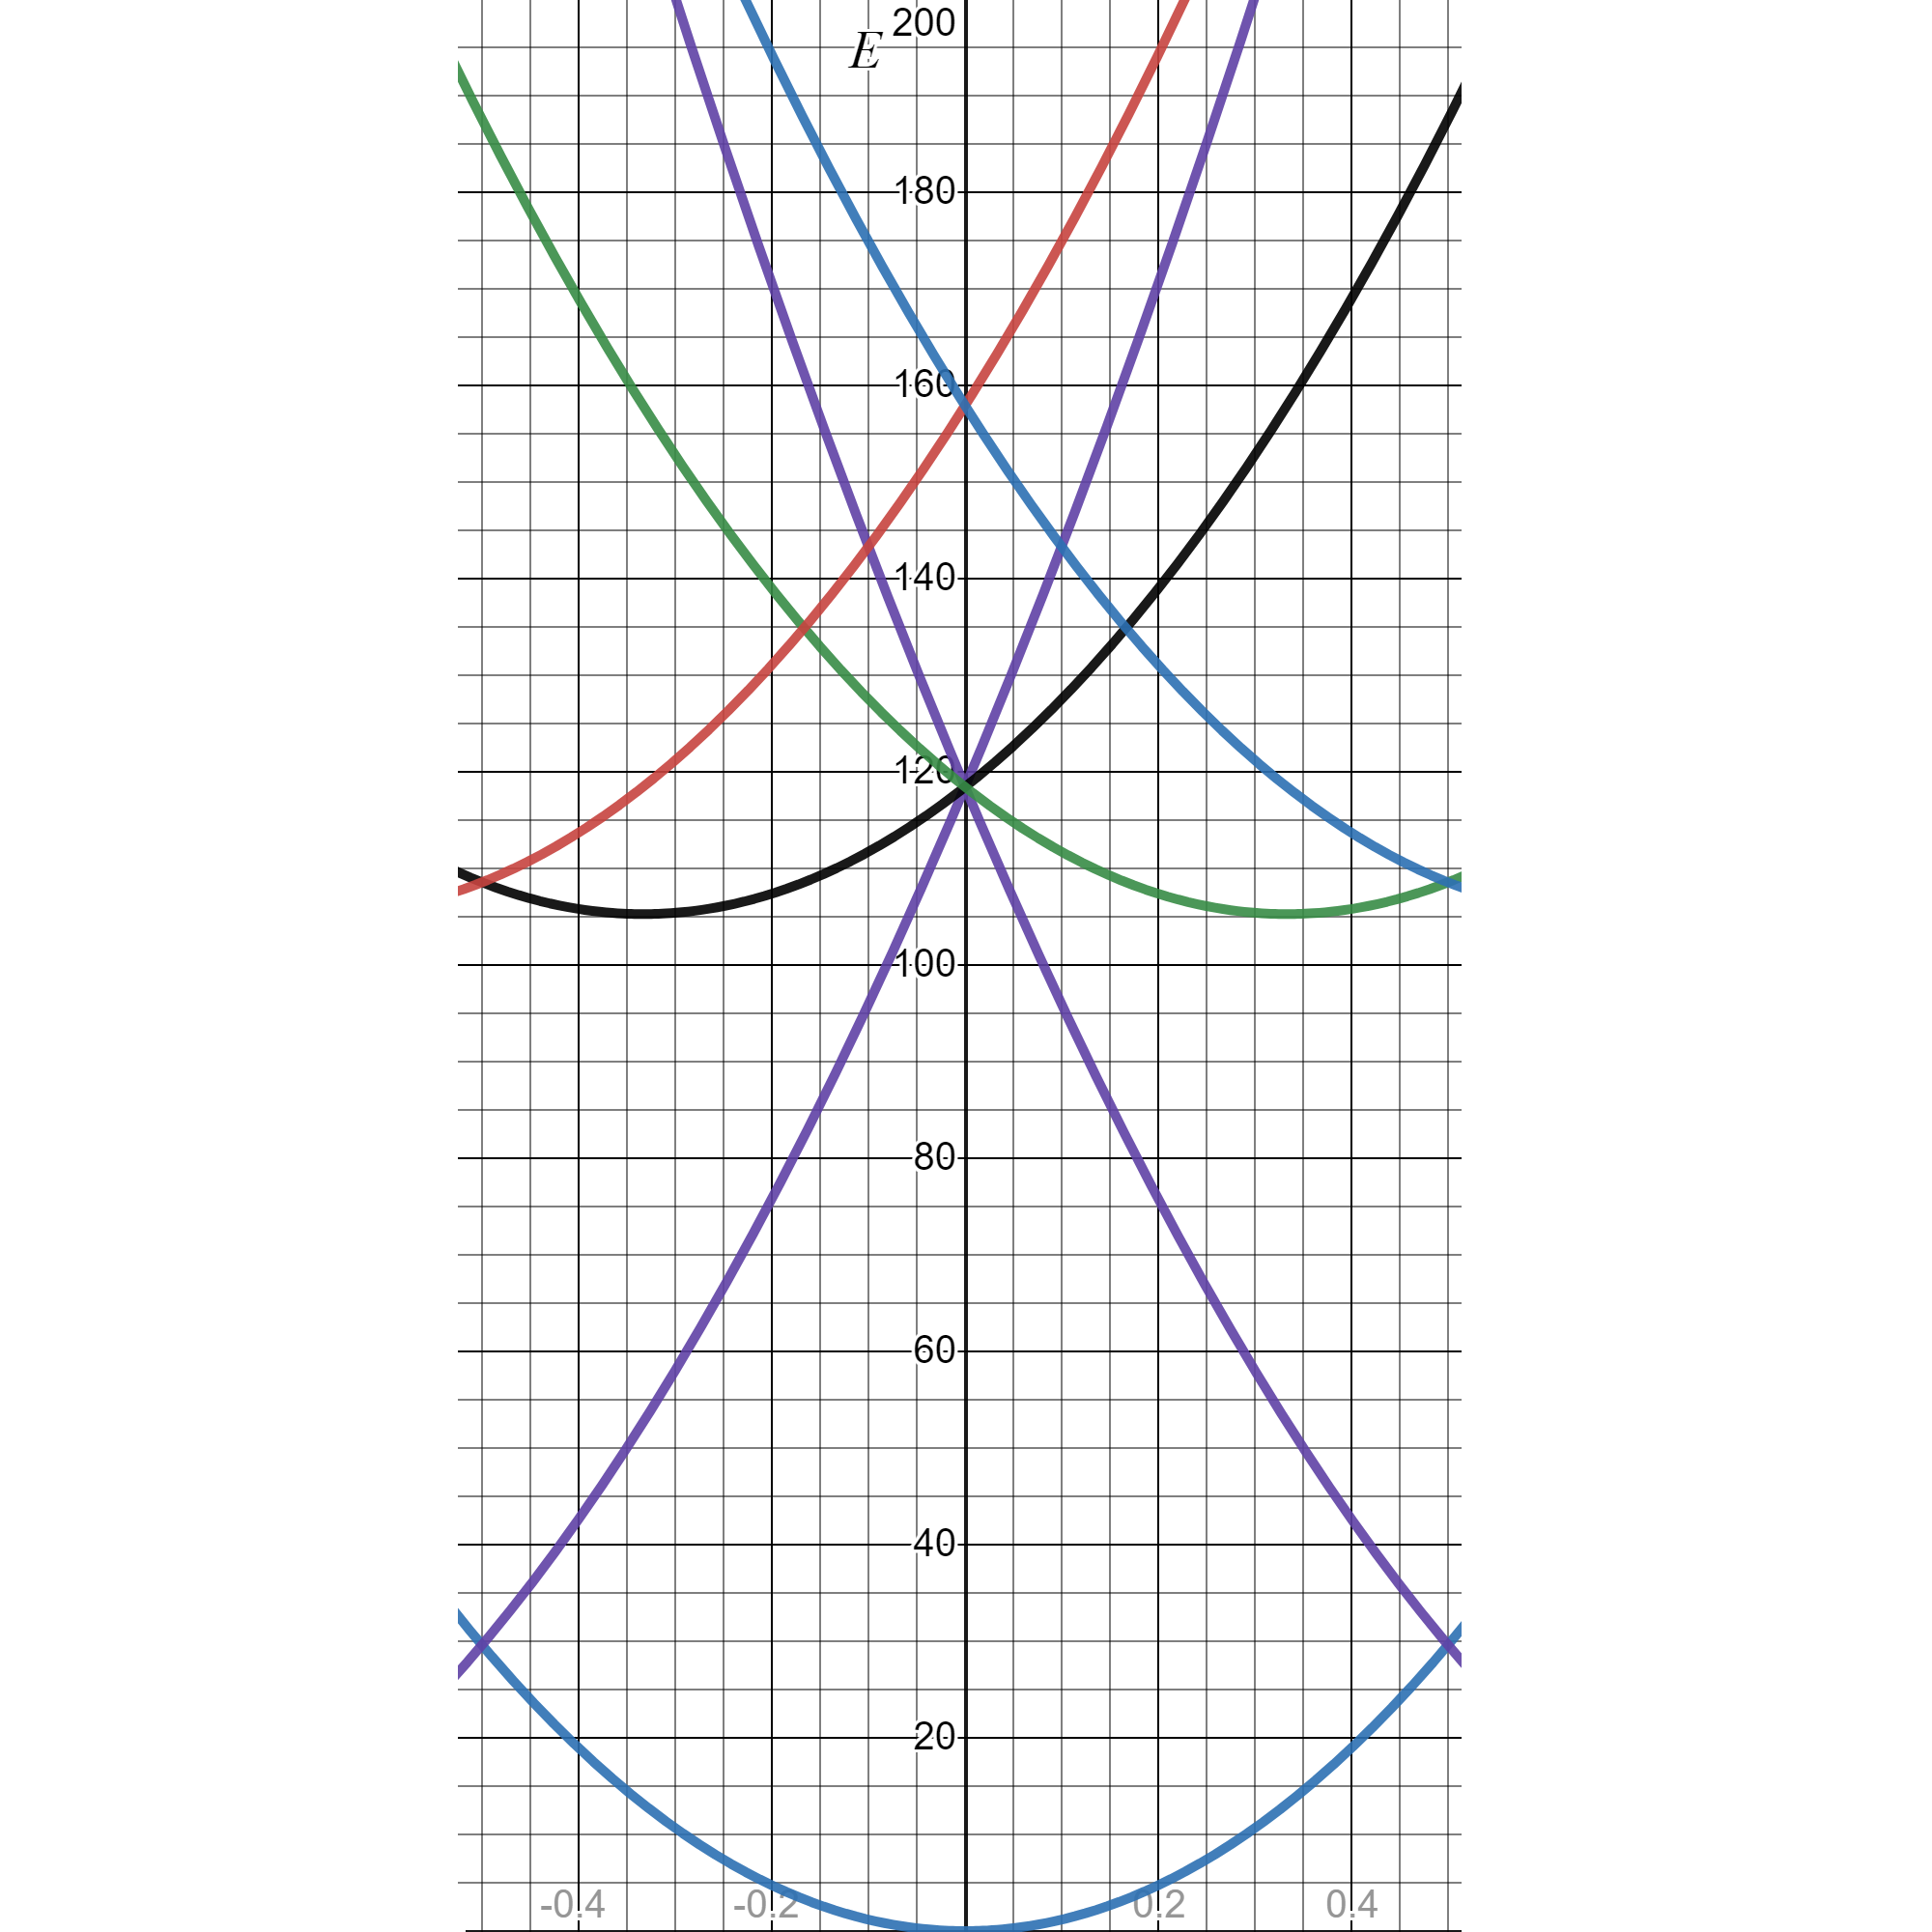
\includegraphics[width=0.9\linewidth]{screenshot001}
			\end{center}
			
			
			
		\pagebreak

		\item % 7.3
			\textbf{\textit{Kronig-Penney model.}} \begin{enumerate}
				\item For the delta-function potential and with $P \ll 1$, find at $k=0$ the energy of the lowest energy band.
				
					\solution For $k=0$, we can reduce eq. (21b) to $$(P/Ka) \sin Ka + \cos Ka = 1.$$
					For $P\ll 1$, the denominator should follow $Ka \ll 1$ to have a valid solution. We can expand the Taylor series to the second order,
					\begin{align*}
						1 & = (P/Ka) \left[Ka + 0 - \dots\right] + \left[1 - (Ka)^2 / 2 + \dots \right] \\
						\implies P & \approx (Ka)^2 / 2.
					\end{align*}
					The associated energy is \begin{align*}
						E & = \hbar^2 K^2 / 2m \tag{13} \\
							& = \hbar^2 P / m  a^2.
					\end{align*}
						
				
				\item For the same problem, find the band gap at $k=\pi/a$.
				
					\solution Similarly, at $k=\pi/a$, eq. (21b) reduces to $$(P/Ka) \sin Ka + \cos Ka = -1.$$
					Then, \begin{align*}
						-1 & = (P/Ka) Ka + 1 - (Ka)^2 / 2 \\
						-2 & = P - (Ka)^2 / 2 \\
						P & \approx (Ka)^2 / 2 + 2. \\
						K^2 & \approx (P - 2) / a^2.\\
						\implies E & =  \hbar^2 K^2 / 2m \\
							& = \hbar^2(P-2) / 2 m a^2.
					\end{align*}
			\end{enumerate}
		
		\pagebreak
		
		\item % 7.4
			\textbf{\textit{Potential energy in the diamond structure.}} \begin{enumerate}
				\item Show that for the diamond structure, the Fourier component $U_G$ of the crystal potential seen by an electron is equal to zero for $\bvec{G}=2\bvec{A}$, where $\bvec{A}$ is a basis vector in the reciprocal lattice referred to the conventional cubic cell.
				
					\solution
					% pp. 16
					Using the diamond structure description on p. 16, the crystal has two atoms at $(0, 0, 0)$ and $(1/4, 1/4, 1/4)$. Then the direct lattice potential is\begin{align*}
						U(x, y, z) & = u(x, y, z) + u(x + 1/4, y + 1/4, z + 1/4),
						\intertext{for a single potential atom potential $u$. In Fourier space, this corresponds to a scaled phase, i.e. $\mathcal{F}\{f(t + k)\} \to  e^{i \omega k} F(\omega)$,}
						U_G & = u_G + u_G e^{iGa/4}.
						\intertext{For $G=2A$, the reciprocal lattice potential is}
						U_G & = u_G \left(
							1 +
							e^{i(Aa) / 2}
						\right).
						\intertext{If $A$ is a basis vector, then we can assume $Aa$ is over a full cycle, so}
						U_G & = u_G ( 1 - 1) = 0. \qed
					\end{align*}
				\item Show that in the usual first-order approximation to the solutions of the wave equation in a period lattice, the energy gap vanishes at the zone boundary plane normal to the end of the vector $\bvec{A}$.
				
					\solution I'm not really sure if I understand this problem correctly. I'm assuming we can get the energy gap from the central equation, but $U=0$ from part (a), so following p. 176--179, we're left with 
					$$(\lambda - \epsilon)^2 = U^2 = 0.$$
					This would mean the energies are $$\epsilon = \lambda \pm 0,$$
					i.e. the energy gap is just zero.
			\end{enumerate}
		
		\pagebreak
		
		\item % 7.6
			\textbf{\textit{Square lattice.}} Consider a square lattice in two dimensions with the crystal potential
			$$U(x, y) = -4 U \cos(2 \pi x / a) \cos(2 \pi y/a).$$
			Apply the central equation to find approximately the energy gap at the corner point $(\pi/a, \pi/a)$ of the Brillouin zone. It will suffice to solve a $2 \times 2$ determinantal equation.
			
			\solution Following what we did in-class, we can first rewrite the potential in complex form, \begin{align*}
				U(x, y) & = -2U_0 \left[\cos(2\pi(x-y)/a) + \cos(2 \pi(x+y)/a) \right] \\
					& = -U_0 \left[
						e^{-i 2 \pi (x - y) / a}
						+ e^{i 2 \pi (x - y) / a}
						+ e^{-i 2 \pi (x + y) / a}
						+ e^{i 2 \pi (x - y) / a}
					\right].
				\intertext{Then we can identify the reciprocal lattice vectors as}
				G & = \{
					(-2 \pi / a, - 2 \pi / a), 
					(2 \pi / a, - 2 \pi / a), 
					(-2 \pi / a, 2 \pi / a), 
					(2 \pi / a, 2 \pi / a)
				\}.
			\end{align*}
			Applying the central equation (27) at $k=(\pi/a, \pi/a)$, \begin{align*}
				(\lambda_k - \epsilon) C(k) + \sum_G U_G C(k - G) & = 0 \\
				(\lambda_k - \epsilon)  C_k 
					+ U_0 C_{(3\pi/a, 3 \pi/a)}
					+ U_0 C_{(3\pi/a, \pi/a)} & \\
					+ U_0 C_{(\pi/a, 3\pi/a)}
					+ U_0 C_{(-\pi/a, -\pi/a)}					
					& = 0.
				\intertext{Dropping the ``far-away'' terms, we're left with}
				(\lambda_k - \epsilon) C_k + U_0 C_{(-\pi/a, -\pi/a)} & = 0.
				\intertext{Next, applying the central equation at $k=(-\pi/a, -\pi/a)$,}
				(\lambda_{-k}  - \epsilon) C_{-k} + U_0 C_{(\pi/a, \pi/a)} & = 0.
			\end{align*}
			Substituting in $$
				\lambda_{\pm k} = \hbar^2 k^2 / 2m = \hbar^2 (2 \pi^2 / a^2) / 2m = \hbar^2 \pi^2 / ma^2,
			$$
			we're left with the coupled equations, \begin{align*}
				(\hbar^2 \pi^2 / ma^2 - \epsilon) C_{(\pi / a, \pi/a)} + U_0 C_{(-\pi / a, - \pi / a)} & = 0 \\
				(\hbar^2 \pi^2 / ma^2 - \epsilon) C_{(\pi / a, \pi/a)} + U_0 C_{(\pi / a, \pi / a)} & = 0.
			\end{align*}
			In determinantal form of $(C_{(\pi/a, \pi/a)}, C_{(-\pi/a, -\pi/a)})$, \begin{align*}
				\begin{vmatrix}
					\hbar^2 \pi^2 / ma^2 - \epsilon & U_0 \\
					U_0 & \hbar^2 \pi^2 / 2ma^2 - \epsilon
				\end{vmatrix} & = 0.
				\intertext{Then,}
				\left(
					\frac{\hbar^2 \pi^2}{ma^2} - \epsilon
				\right)^2 & = U_0^2.
			\end{align*}
			Removing the square and solving for the energies of each \begin{align*}
				\epsilon & = \frac{\hbar^2 \pi^2}{ma^2} \mp U_0 \\
				\text{Gap energy} & = 2 U_0.
			\end{align*}
	\end{enumerate}
\end{document}